% --
% Neural Network Architectures

\chapter{Neural Networks}\label{sec:nn}
%This chapter contains theoretical foundations and practical evaluation of developing a Key Word Spotting (KWS) system with neural networks, especially intended for video games
This chapter contains theoretical foundations and practical results regarding neural networks applied to the key word spotting in classifying speech commands.
The used architectures within this thesis are shown and explained in detail.
The training of those networks and some special concepts, such as adversarial pre-training, are presented.
Special focus is lied on energy efficiences, because key word spotting requires it in many practical applications, such as well as video games.


% theory
% --
% theory

\section{Theory}\label{sec:nn_theory}
This section provide the preliminaries to understand the used neural network architectures and the training procedure in general.


% activation functions
\subsection{Activation Functions}\label{sec:nn_theory_acti}
Activation functions for neural networks are non-linear functions that map the sum of the weighted inputs to an output value of a node:
\begin{equation}\label{eq:nn_theory_acti}
  z = h(w \, x^T)
\end{equation}
where $h$ is the activation function, $w \in \R^n$ is an weight vector and $x \in \R^n$ an input vector for one specific node.
One constraint of an activation function is, that an easy computable derivative of this function exist, such that the backpropagation of gradients work.


% cnn
\subsection{Convolutional Neural Networks}\label{sec:nn_theory_cnn}
Covolutional Neural Networks (CNN) as already discussed in \rsec{prev_nn_cnn} use convolutional filters on spatial sections of the input.
Those convolutional filters are also called kernels, for images illustrated as rectangle in 2D space with kernel width $k_w$ and height $k_h$.

The kernel is shifted over its input map in each axis with an operation called \emph{stride}, denoted as $s$, and produce a output map.
The output dimension $o_d$ for striding in along its axis with $s_d$ and kernel size for that axis $k_d$ over the input dimension $i_d$ can be computed as:
\begin{equation}\label{eq:nn_theory_cnn_}
  o_d = \floor*{\frac{i_d + p_d - k_d}{s_d} + 1}
\end{equation}
where $p_d$ is additionally a \emph{padding} term, where for instance for in zero-padding, zeros are added on both sides of the input dimension.
For example if a $16 \times 16$ image is convoluted by a $5 \times 5$ kernel with stride $1$ in each direction and no padding, the output image is $12 \times 12$.
The padding operation has usually the purpose to keep a the output and input dimension the same.
This is used for instance in residual neural networks, where the input to convolutional layers of a block, is bypassed and added to the output of this block again.
Being able to compute the addition operation from input and output of the residual block, their dimensions must be the same.
However in most usual convolutional network applications without residual blocks, it is preferred not to pad the image, so that dimensions are reduced hence parameters and multiplications saved.
Further there exist special convolutional layers that should reduce the dimensions, such as a Max-Pooling layers. 

As already mentioned above CNNs are defined with the amount of input and output channels (feature maps), the kernel size, the stride of the kernel and some other specialties like dilation.
However it is not immediately clear from those parameter, how many convolutional filters are applied and what how the output feature maps are calculated.
Usually in most applications, the convolution to output feature maps are done with:
A typical example is shown in...

\begin{figure}[!ht]
  \centering
    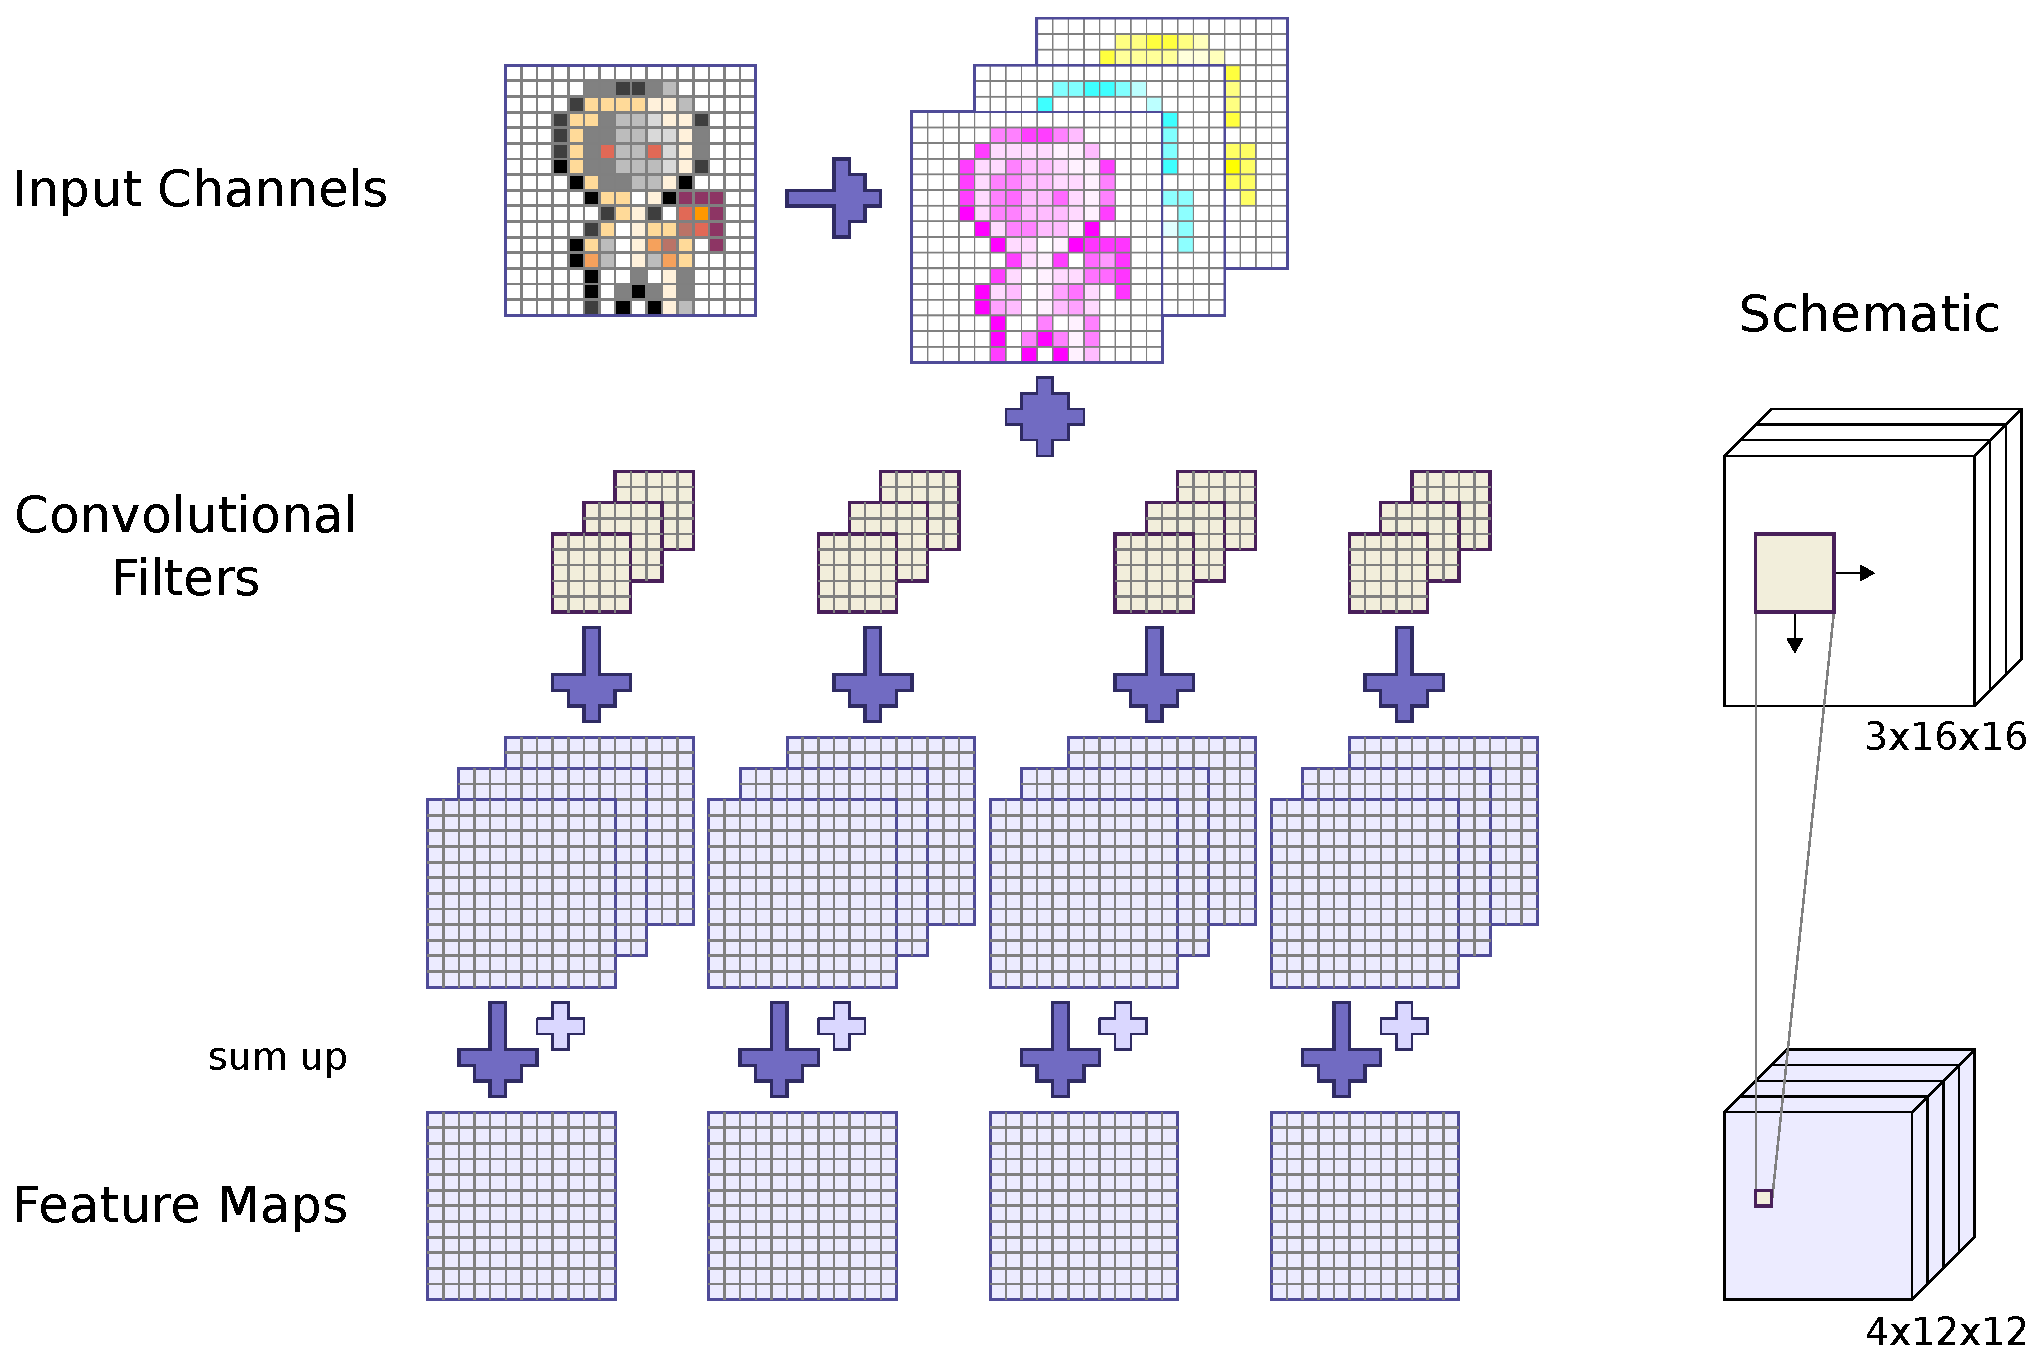
\includegraphics[width=0.6\textwidth]{./4_nn/figs/cnn_basics.eps}
  \caption{CNN basic architecture}
  \label{fig:nn_theory_cnn_basics}
\end{figure}
\FloatBarrier
\noindent

% \begin{figure}[h]
%   \centering{
%   \resizebox{0.5\textwidth}{!}{\input{./4_nn/figs/cnn_basics.tex}}}
%   \caption{CNN basic architecture}
%   \label{fig:nn_theory_cnn_basic}
% \end{figure}
% \FloatBarrier
% \noindent


% architectures
% --
% Neural Network Architectures

\section{Neural Network Architectures}\label{sec:nn_arch}
All Neural Network Architectures evaluated within this thesis are presented here.
%There will be a general classification between Neural Network Architectures by Convolutional Neural Networks, Adversarial Neural Networks ...
In general the architectures can be differentiated between:
\begin{enumerate}
	\item Convolutional Neural Networks
	\item Adversarial Neural Networks
	\item Wavenets
\end{enumerate}
The term Convolutional Neural Networks here consists of all architectures consisting of at least one convolutional layer and the intention to simply classify each speech commands from each other. 
Therefore the output of a Convolutional net is of size of the amount of speech commands and usually has some kind of probability distribution or energy equivalence.

With Adversarial Neural Networks all architectures are meant, with at least two separate Neural Network Architectures, e.g. a Discriminator and a Generator Network and the intention to outperform the other Network in a task where both play a game against each other.
The word game here, is used in the sense of Game Theory, where the goal is to find an equilibrium state where both players are equally satisfied with the state.

An overview of all models is shown in \rtab{nn_arch_overview} with abbreviations in \rtab{nn_arch_abbreviation}.
\begin{table}[ht!]
\begin{center}
\caption{Network Architectures Abbreviations}
\begin{tabular}{ M{2.5cm}  M{10cm} }
\toprule
\textbf{Abbreviations} & \textbf{Meaning}\\
\midrule
c[0-9] & convolutional layer with layer number\\
f[0-9] & feed forward fully connected layer with layer number\\
m[0-9] & max pooling layer layer with layer number\\
ch & input channel number for mfccs it is usually 1\\
fs & frame size (usually 50 -> 50ms)\\
ms & feature size (mfcc), depends on feature selection\\
cf & output number of last flattened convolutional layer\\
cl & number of class labels\\
\bottomrule
\label{tab:nn_arch_abbreviation}
\end{tabular}
\end{center}
\end{table}
\FloatBarrier
\noindent
\begin{table}[ht!]
\begin{center}
\caption{Network Architectures Overview with reference names}
\begin{tabular}{ M{2.5cm}  M{2.1cm}  M{2.1cm} M{2.1cm} M{2.5cm}}
\toprule
%\multicolumn{4}{c}{\textbf{Feature Groups}} & \multicolumn{2}{c}{\textbf{Accuracy}} \\
\textbf{Reference name} & \textbf{Feature maps} & \textbf{Kernel sizes} & \textbf{Strides} & \textbf{Feed Forward} \\
\midrule
conv-trad & c1: (ch, 64) c2: (64, 64) & c1: (4, 20) mp: (2, 4) c2: (2, 4) & c1: (1, 1) mp: (2, 4) c2: (1, 1) & f1: (cf, 32) \quad f2: (32, 128) f3: (128, cl)\\
\midrule
conv-fstride & c1: (ch, 54) & c1: (8, fs) & c1: (4, 1) & f1: (cf, 32) \quad f2: (32, 128) \quad f3: (128, 128) \quad f4: (128, cl)\\
\midrule
conv-encoder-fc1 & c1: (ch, 48) \quad c2: (48, 8) & c1: (ms, 20) \quad c2: (1, 5) & c1: (1, 1) \quad c2: (1, 1) & f1: (cf, cl)\\
\midrule
conv-encoder-fc3 & c1: (ch, 48) \quad c2: (48, 8) & c1: (ms, 20) \quad c2: (1, 5) & c1: (1, 1) \quad c2: (1, 1) & f1: (cf, 64) \quad f2: (64, 32) \quad f3: (32, l)\\
\bottomrule
\label{tab:nn_arch_overview}
\end{tabular}
\end{center}
\end{table}
\FloatBarrier
\noindent



% adversarial
% --
% adversarial

\section{Adversarial Training Theory}\label{sec:nn_adv}
Working with adversarial Neural Networks is quite interesting, as two separate Networks are challenge themselves against each other to improve their performance.
The paper from Goodfellow et. al. \cite{Goodfellow2014} describes a game between two Neural Networks (players), where one player has the role of creating fakes and the other must determine if it is real or fake.
The Network who creates fakes is called Generator (G) and the other Network who has to decide about fake or not is called Discriminator (D).
The Generators goal is to create fakes that look like reals, so that D makes mistakes and classifies a fake as a real.
On the other hand the Discriminator must also constantly improving itself, so that fakes from G can be detected and sorted out from the reals.

This approach works remarkably well to create a generative network able to produce fakes that are astonishing similar to real ones.
In the mentioned paper, this was applied to images and not for audio data.
But if the audio waveform is presented as spectogram or mfcc with fixed frame size, it can be seen as an image, where one dimension is time and the other frequency.

So far a generative network does only produce fake images and a discriminative network can only output a one dimensional (probability) output, to decide if it is fake or not.

The idea now is not to use either of these networks, but to use transfer learning in the sense to reuse the convolutional layers both networks achieved during their game (training).
The weights of those convolutional layers are then transfered to another network with classification purpose on multiple labels.

\subsection{Questions that arise}
There are several questions that arise regarding Adversarial Training:
\begin{enumerate}[label={Q.\textgoth{A}.\arabic*)}, leftmargin=1.4cm]
  \item Does the Network Architecture of G and D have to be the same but transposed?
  \item Does the value space of in and outputs, for D and G respectively, have to be limited e.g. [0, 1] done by e.g. frame normalization, or sigmoid output?
  \item What loss function works well for training?
  \item How long should be trained?
  \item When transfering weights to another network, should the weights from G or D be transfered?
  \item Does the classification network has to adapt the parameters from the transfered weights?
  \item Whats the benefit of all this?
\end{enumerate}

To illustrate the idea an example is shown of the labels L5 (left, right, up, down, go).

The convolutional layer weights from the adversarial training of the individual labels, 
can be stacked together an used to initialize another network.
An example of this method is shown in \rfig{nn_adv_example}, where the initialization pattern changes to more elaborate structures and patterns to form good classification outputs. 
However the Basic Pattern from the adversarial training stays the same, which is a good sign, because then the network is accepting those trained weights and adapts them.

\begin{figure}[!ht]
  \centering
    \subfigure[c1 trained]{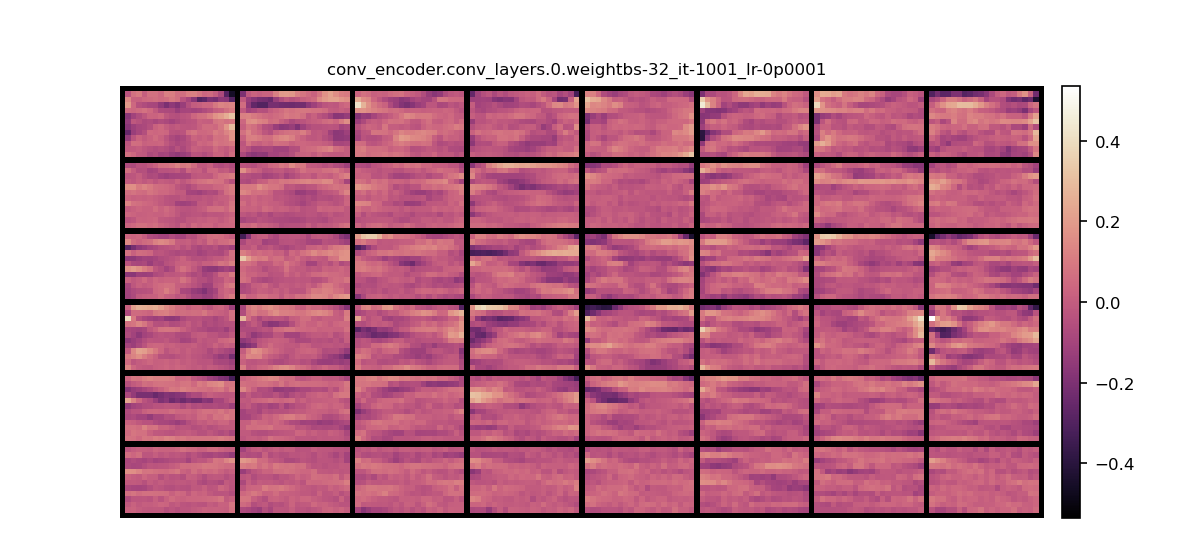
\includegraphics[width=0.45\textwidth]{./4_nn/figs/nn_adv_example_c0}}
    \subfigure[c1 init]{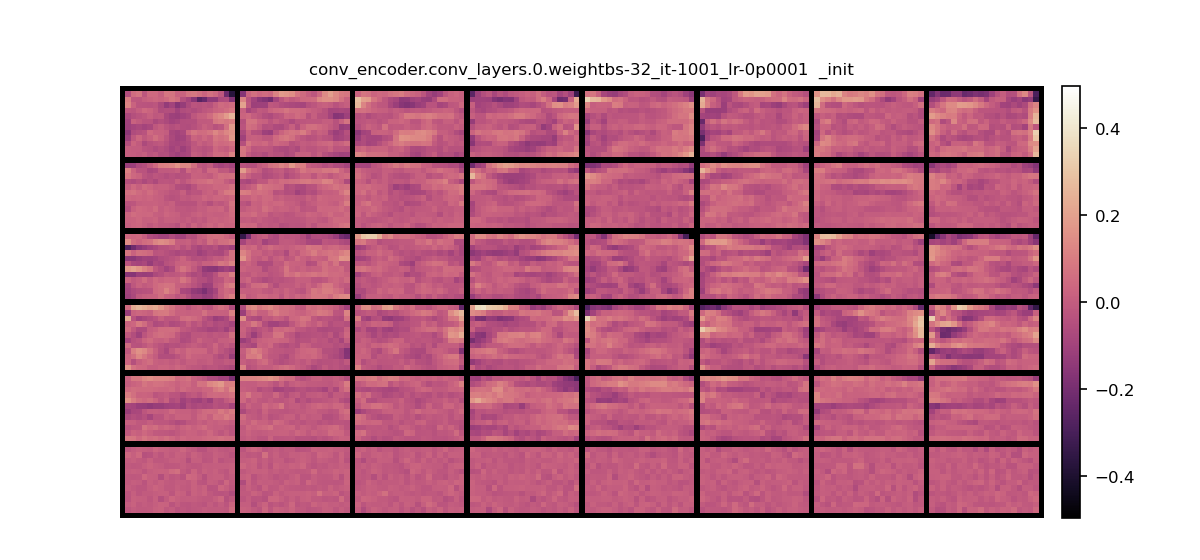
\includegraphics[width=0.45\textwidth]{./4_nn/figs/nn_adv_example_c0_init}}
    \subfigure[c2 trained]{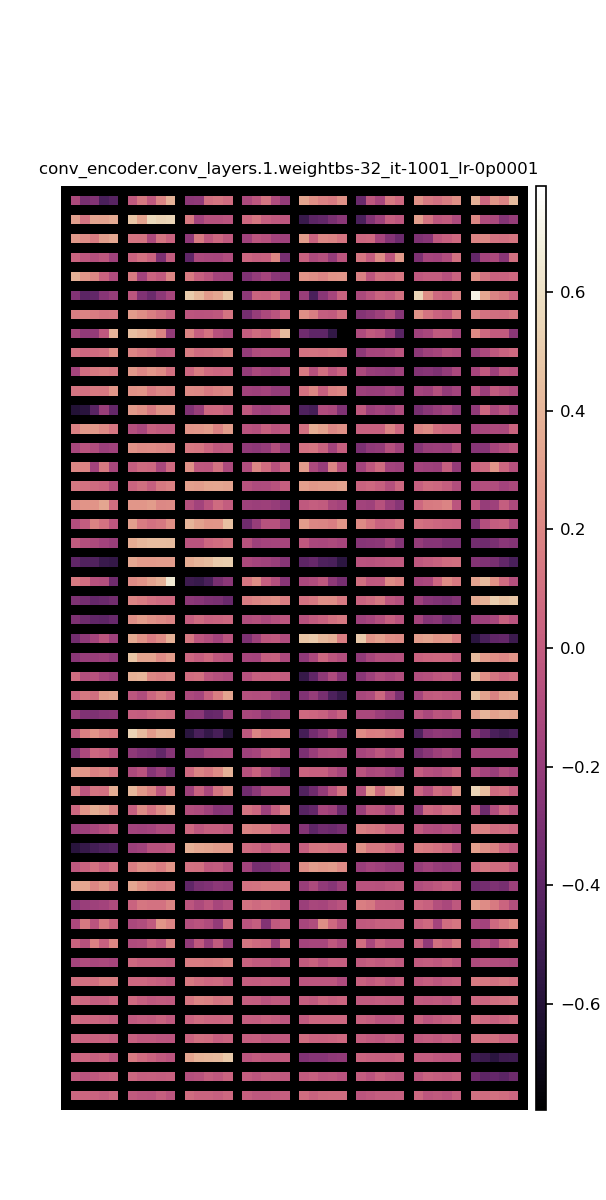
\includegraphics[height=0.45\textwidth]{./4_nn/figs/nn_adv_example_c1}}
    \quad
    \subfigure[c2 init]{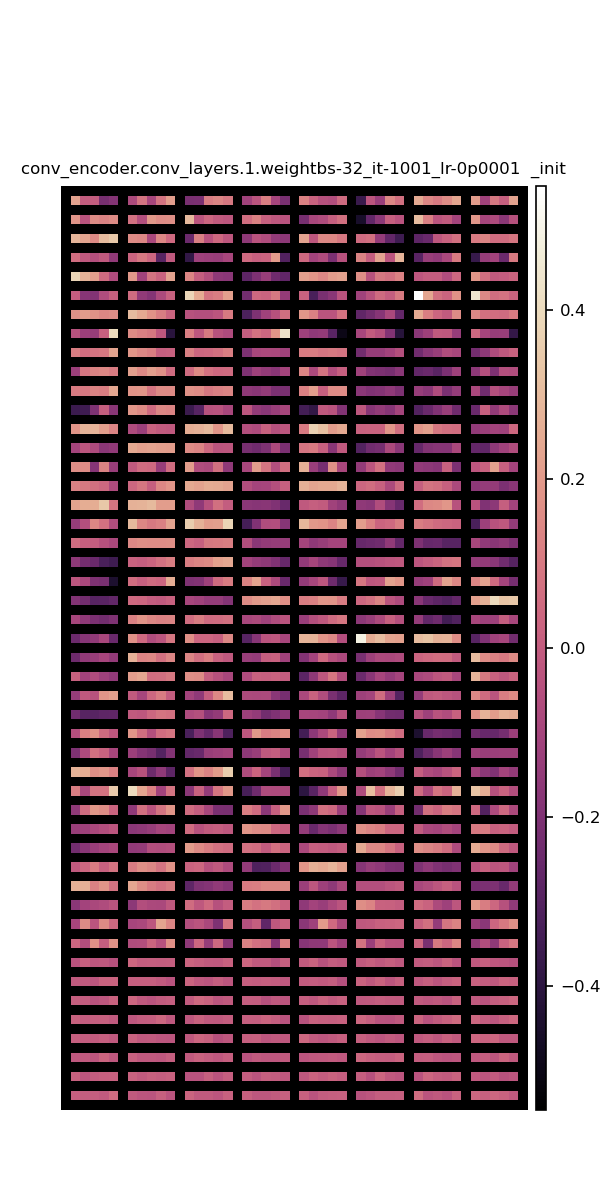
\includegraphics[height=0.45\textwidth]{./4_nn/figs/nn_adv_example_c1_init}}
  \caption{Adversarial Training Example: Convolutional layers pretrained with adversarial training on each label separately.}
  \label{fig:nn_adv_example}
\end{figure}
\FloatBarrier
\noindent

For this example in adversarial training, 8 feature maps of the first layer were used for each label, also they belong to the Generator Network G or decoder (dec). In Convolutional Networks, each previous layers feature map creates a new set of feature maps in the next layer.
An example of this label training is shown in \rfig{nn_adv_example_label} with feature maps [(1, 8), (8, 8)] of the convolutional layers

\begin{figure}[!ht]
  \centering
    \subfigure[\enquote{left} c1 from D]{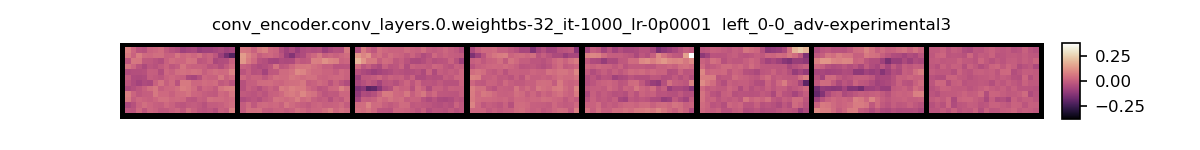
\includegraphics[width=0.45\textwidth]{./4_nn/figs/nn_adv_example_label_left_c0_enc}}
    \subfigure[\enquote{left} c1 from G]{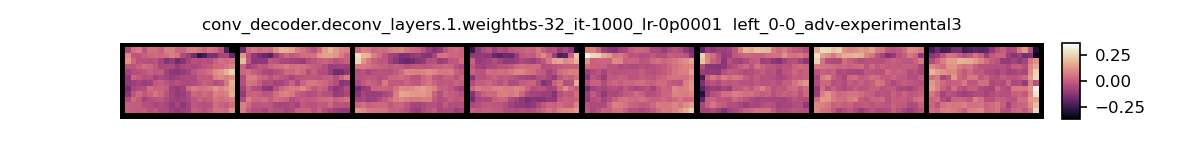
\includegraphics[width=0.45\textwidth]{./4_nn/figs/nn_adv_example_label_left_c0_dec}}
    \subfigure[\enquote{left} c2 from D]{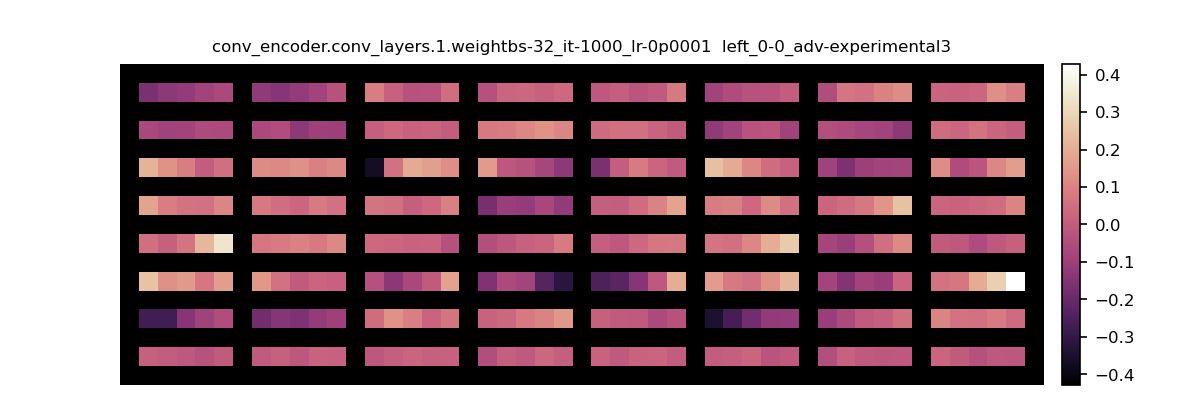
\includegraphics[width=0.3\textwidth]{./4_nn/figs/nn_adv_example_label_left_c1_enc}}
    \subfigure[\enquote{left} c2 from G]{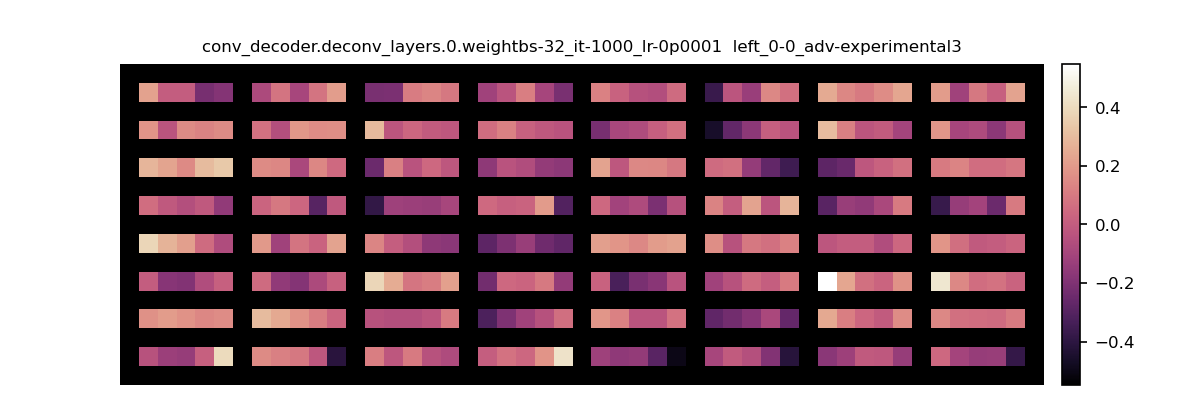
\includegraphics[width=0.3\textwidth]{./4_nn/figs/nn_adv_example_label_left_c1_dec}}
  \caption{Adversarial Training example of Generator (G) and Discriminator (D) of label \enquote{left} captured with 8 feature maps of the first convolutional layer.}
  \label{fig:nn_adv_example_label}
\end{figure}
\FloatBarrier
\noindent

Those trained weights from each label can then simply be put into the feature maps of a classification network.
This is shown in \rfig{nn_adv_example} where c1 from G and c2 from G in \rfig{nn_adv_example_label} were transfered to the first row(s).
When doing the transferring of feature maps, it is important that the layers are not mixed up so that the trained connections are still correct.
Also of course the weights of the feature maps must have the same dimension, so that transferring is possible.


\subsection{Observing the Generators output}
While the output of the Discriminator is rather uninteresting (one-dimensional probability value), the output of the Generator is a good indicator of how well the training between D and G has gone.
Optimally the output of the Generator look like real data samples.
An example of a trained Generator Network with fake outputs compared to real ones is shown in \rfig{nn_adv_gen}.

\begin{figure}[!ht]
  \centering
    \subfigure[\enquote{left} real examples]{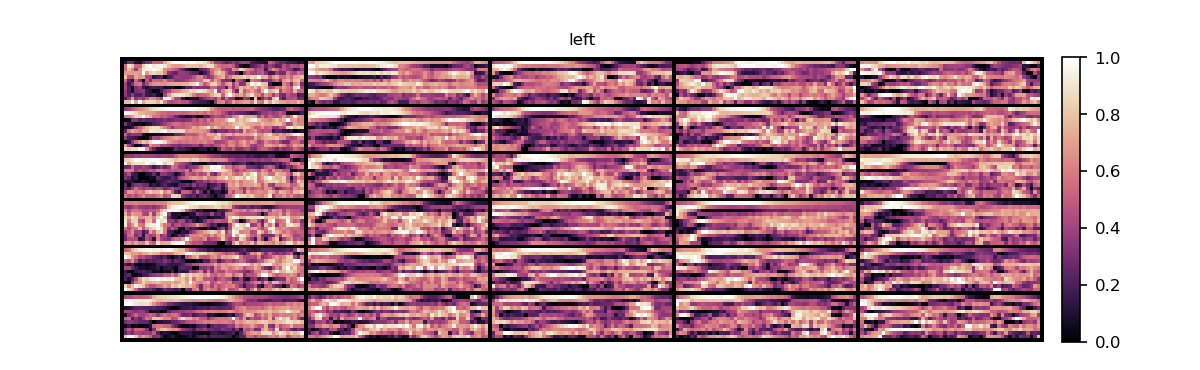
\includegraphics[width=0.45\textwidth]{./4_nn/figs/nn_adv_gen_left_real}}
    \subfigure[\enquote{left} fakes from G]{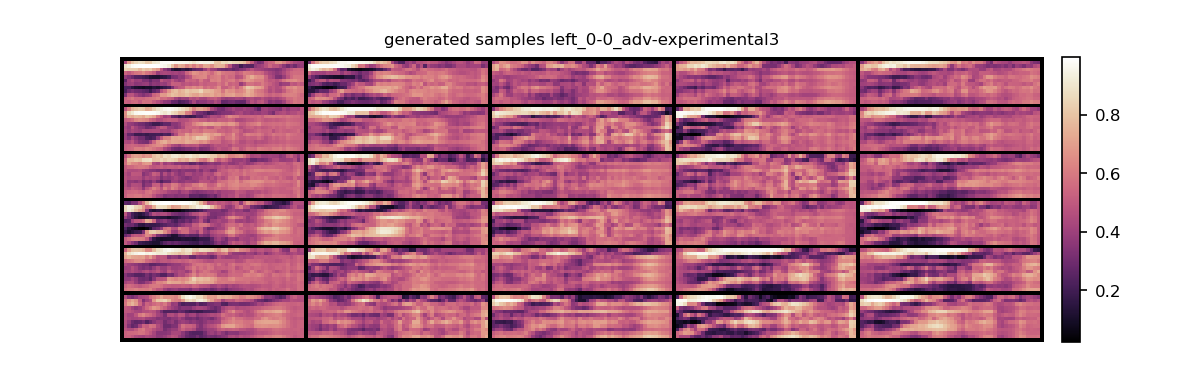
\includegraphics[width=0.45\textwidth]{./4_nn/figs/nn_adv_gen_left_fake}}
  \caption{Real samples of \enquote{left} from the Speech Commands dataset compared to fake samples from a trained Generator Network.}
  \label{fig:nn_adv_gen}
\end{figure}
\FloatBarrier
\noindent

If the fake example of the Generator Network do not look similar to real ones, then something might have gone wrong in the training between the Generator and Discriminator Network.
Further it can be evaluated if a certain network architecture is able to produce a label in a sufficient representation, therefore this method might be a good start in finding a suitable network architecture for the problem to be solved.



